% arara: pdflatex
% arara: biber
% arara: makeindex
% arara: nomencl
% arara: pdflatex
% arara: pdflatex

\documentclass[a4paper,12pt]{article}
%\RequirePackage[l2tabu,orthodox]{nag}

\usepackage{upreport}
\usepackage{tabularx}
\usepackage{amssymb}
\usepackage{siunitx}
\addbibresource{report.bib}
\title{Project Process and  Model Description}
\subject{CBT 700}
\date{\today}

%Nomenclature unit command
\newcommand{\nomunit}[1]{%
\renewcommand{\nomentryend}{\hspace*{\fill}#1}}

% Create a custom user command or run the following 
%  makeindex %.nlo -s nomencl.ist -o %.nls
% execute this command after compiling your file once, then compile a second time to generate a nomenclature table



\begin{document}
\maketitle

\section{System Diagram}

The Process Flow Diagram of the system, with all the relevant inputs, outputs and disturbances are displayed in Figure~\ref{fig:PFD}.

\begin{figure}[tbph]
	\centering
	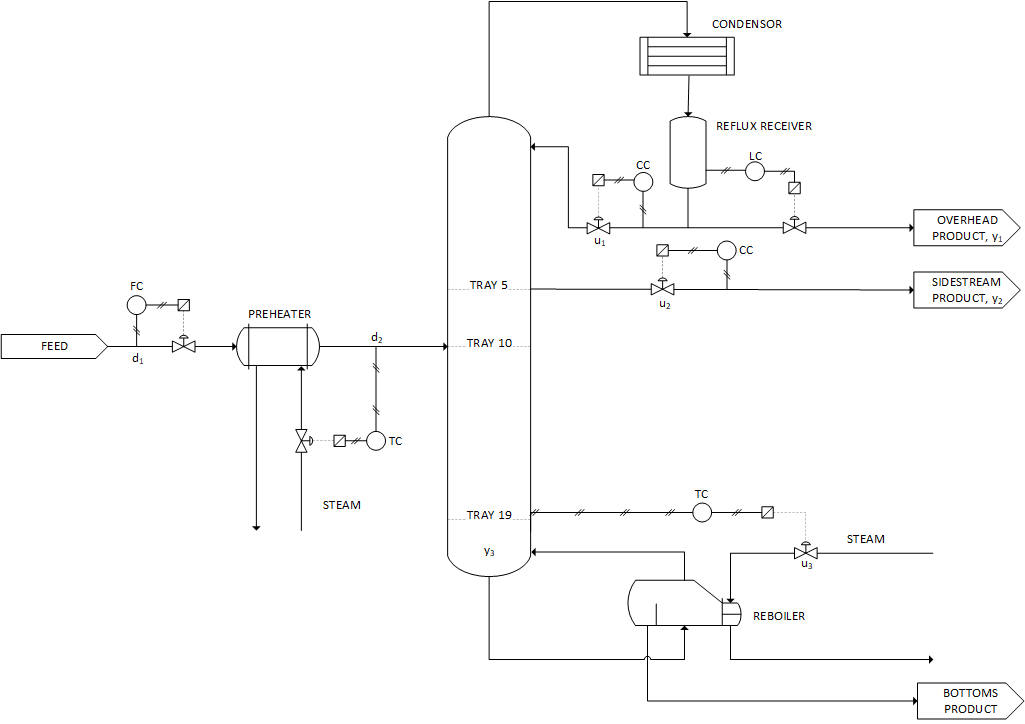
\includegraphics[width=0.9\linewidth]{../Process_PFD}
	\caption{Process flow diagram of the system}
	\label{fig:PFD}
\end{figure}

\newpage
\section{System Description}

The system involves the separation of water and ethanol (in a solution), with the aim of producing an ethanol product that can be used as an alternative fuel source.

The distillation column studied is a 19 tray, 12 inch diameter column. The column has variable feed and side stream draw off locations. The side stream flow is varied to control the composition of the stream. The distillate vapour draw off stream is fully condensed, and then separated into the reflux and product streams. The product stream is set to control the level in the condenser, while the reflux stream controls the composition of the distillate product. A kettle re-boiler is used to add energy to the column. Stream is the main utility. The amount re-boiled bottoms product is controlled by varying the steam supplied to the re-boiler. The feed temperature and flow rate can be controlled to simulated disturbances on the system. These variables are strictly defined as disturbances.

The compositions are measured/determined through various on-line sensors (densitrometry and refractometry).

Currently all variables are controlled with single input single output (SISO) control loops.

\newpage
\section{System Variables}

\begin{table}[h]
	\label{teb:Variables}
	\centering
	\caption{Summary of all the model variables.}
	\begin{tabular}{cccc}
		\hline
		\multicolumn{4}{c}{Input Variables}                                       \\
		
		Variable & Description                       & Steady State Value & Units \\
		\hline
		$u_1$       & Reflux flow rate                  & 0.18               & gpm   \\
		$u_2$       & Side stream product flow rate     & 0.046              & gpm   \\
		$u_3$       & Reboiler steam pressure           & 20                 & psi   \\
		\hline
		\multicolumn{4}{c}{Output Variables}                                      \\
		
		Variable & Description                       & Steady State Value & Units \\
		\hline
		$y_1$       & Overhead ethanol mole fraction    & 0.7                & -     \\
		$y_2$       & Side stream ethanol mole fraction & 0.52               & -     \\
		$y_3$       & Tray \#19 temperature             & 92                 & \si{\celsius} \\
		\hline
		\multicolumn{4}{c}{Disturbance Variables}                                 \\
		
		Variable & Description                       & Steady State Value & Units \\
		\hline
		$d_1$       & Feed flow rate                    & 0.8                & gpm   \\
		$d_2$       & Feed temperature                  & 78                 & \si{\celsius} \\\hline
	\end{tabular}
\end{table}

\newpage
\section{System Model}

The model was determined by conducting pulse testing on the system. In most case a first order plus dead time model gave a sufficiently accurate fit to experimental data (based on the sum of the squared error method). In some cases, a second order system with first order lag and dead time, was used to accurately describe the impulse response. The fitting curves of two pulse tests are displayed in Figure~\ref{fig:test1} and Figure~\ref{fig:test2}.

\begin{figure}[htbp]
	\centering
	\begin{minipage}{.48\textwidth}
		\centering
		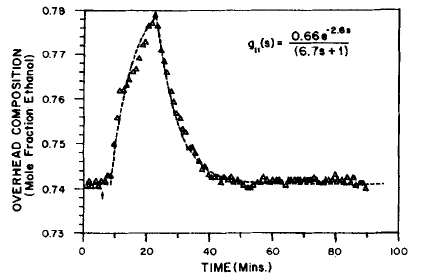
\includegraphics[width=\linewidth]{Figures/Pulse_test_1}
		\captionof{figure}{Overhead composition response to a pulse of 15 minutes duration in the reflux rate.}
		\label{fig:test1}
	\end{minipage}%
	\hfill
	\begin{minipage}{.48\textwidth}
		\centering
		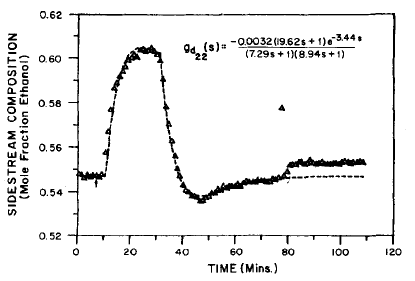
\includegraphics[width=\linewidth]{Figures/Pulse_test_2}
		\captionof{figure}{Side stream composition response to a pulse of 15 minutes duration in feed temperature.}
		\label{fig:test2}
	\end{minipage}
\end{figure}

The model takes the form of a commonly employed linear model for a MIMO system,

\begin{equation}
\textbf{y}(s) = \textbf{G}(s)\textbf{u}(s) + \textbf{G}_{d}(s)\textbf{d}(s)
\end{equation}

where

\begin{equation}
	\textbf{G}(s) = \begin{bmatrix}
	G_{11} & G_{12} & G_{13} \\
	G_{21} & G_{22} & G_{23} \\
	G_{31} & G_{32} & G_{33} \\
	\end{bmatrix} = \begin{bmatrix}
	\frac{0.66e^{-2.6s}}{6.7s+1} & \frac{-0.61e^{-3.5s}}{8.64s+1} & \frac{-0.0049e^{-s}}{9.06s+1} \\
	\frac{1.11e^{-6.5s}}{3.25s+1} & \frac{-2.36e^{-3s}}{5.0s+1} & \frac{-0.012e^{-1.2s}}{7.09s+1} \\
	\frac{-34.68e^{-9.2s}}{8.15s+1} & \frac{46.2e^{-9.4s}}{10.9s+1} & \frac{0.87(11.61s+1)e^{-s}}{(3.89s+1)(18.8s+1)}
	\end{bmatrix}
\end{equation}

and

\begin{equation}
\textbf{G}_{d}(s) = \begin{bmatrix}
G_{d11} & G_{d12} \\
G_{d21} & G_{d22} \\
G_{d31} & G_{d32} \\
\end{bmatrix} = \begin{bmatrix}
\frac{0.14e^{-12s}}{6.2s+1} & \frac{-0.0011(26.32s+1)e^{-2.66s}}{(7.85s+1)(4.63s+1)} \\
\frac{0.53e^{-10.5s}}{6.9s+1} & \frac{-0.0032(19.62s+1)e^{-3.44s}}{(7.29s+1)(8.94s+1)} \\
\frac{-11.54e^{-0.6s}}{7.01s+1} & \frac{0.32e^{-2.6s}}{7.76s+1}
\end{bmatrix}
\end{equation}


\appendix
\renewcommand{\thefigure}{\thesection.\arabic{figure}}
\renewcommand{\thetable}{\thesection.\arabic{table}}
\renewcommand{\thepage}{\thesection.\arabic{page}}
\end{document}